\documentclass[twoside]{book}

% Packages required by doxygen
\usepackage{fixltx2e}
\usepackage{calc}
\usepackage{doxygen}
\usepackage[export]{adjustbox} % also loads graphicx
\usepackage{graphicx}
\usepackage[utf8]{inputenc}
\usepackage{makeidx}
\usepackage{multicol}
\usepackage{multirow}
\PassOptionsToPackage{warn}{textcomp}
\usepackage{textcomp}
\usepackage[nointegrals]{wasysym}
\usepackage[table]{xcolor}

% Font selection
\usepackage[T1]{fontenc}
\usepackage[scaled=.90]{helvet}
\usepackage{courier}
\usepackage{amssymb}
\usepackage{sectsty}
\renewcommand{\familydefault}{\sfdefault}
\allsectionsfont{%
  \fontseries{bc}\selectfont%
  \color{darkgray}%
}
\renewcommand{\DoxyLabelFont}{%
  \fontseries{bc}\selectfont%
  \color{darkgray}%
}
\newcommand{\+}{\discretionary{\mbox{\scriptsize$\hookleftarrow$}}{}{}}

% Page & text layout
\usepackage{geometry}
\geometry{%
  a4paper,%
  top=2.5cm,%
  bottom=2.5cm,%
  left=2.5cm,%
  right=2.5cm%
}
\tolerance=750
\hfuzz=15pt
\hbadness=750
\setlength{\emergencystretch}{15pt}
\setlength{\parindent}{0cm}
\setlength{\parskip}{3ex plus 2ex minus 2ex}
\makeatletter
\renewcommand{\paragraph}{%
  \@startsection{paragraph}{4}{0ex}{-1.0ex}{1.0ex}{%
    \normalfont\normalsize\bfseries\SS@parafont%
  }%
}
\renewcommand{\subparagraph}{%
  \@startsection{subparagraph}{5}{0ex}{-1.0ex}{1.0ex}{%
    \normalfont\normalsize\bfseries\SS@subparafont%
  }%
}
\makeatother

% Headers & footers
\usepackage{fancyhdr}
\pagestyle{fancyplain}
\fancyhead[LE]{\fancyplain{}{\bfseries\thepage}}
\fancyhead[CE]{\fancyplain{}{}}
\fancyhead[RE]{\fancyplain{}{\bfseries\leftmark}}
\fancyhead[LO]{\fancyplain{}{\bfseries\rightmark}}
\fancyhead[CO]{\fancyplain{}{}}
\fancyhead[RO]{\fancyplain{}{\bfseries\thepage}}
\fancyfoot[LE]{\fancyplain{}{}}
\fancyfoot[CE]{\fancyplain{}{}}
\fancyfoot[RE]{\fancyplain{}{\bfseries\scriptsize Generated by Doxygen }}
\fancyfoot[LO]{\fancyplain{}{\bfseries\scriptsize Generated by Doxygen }}
\fancyfoot[CO]{\fancyplain{}{}}
\fancyfoot[RO]{\fancyplain{}{}}
\renewcommand{\footrulewidth}{0.4pt}
\renewcommand{\chaptermark}[1]{%
  \markboth{#1}{}%
}
\renewcommand{\sectionmark}[1]{%
  \markright{\thesection\ #1}%
}

% Indices & bibliography
\usepackage{natbib}
\usepackage[titles]{tocloft}
\setcounter{tocdepth}{3}
\setcounter{secnumdepth}{5}
\makeindex

% Hyperlinks (required, but should be loaded last)
\usepackage{ifpdf}
\ifpdf
  \usepackage[pdftex,pagebackref=true]{hyperref}
\else
  \usepackage[ps2pdf,pagebackref=true]{hyperref}
\fi
\hypersetup{%
  colorlinks=true,%
  linkcolor=blue,%
  citecolor=blue,%
  unicode%
}

% Custom commands
\newcommand{\clearemptydoublepage}{%
  \newpage{\pagestyle{empty}\cleardoublepage}%
}

\usepackage{caption}
\captionsetup{labelsep=space,justification=centering,font={bf},singlelinecheck=off,skip=4pt,position=top}

%===== C O N T E N T S =====

\begin{document}

% Titlepage & ToC
\hypersetup{pageanchor=false,
             bookmarksnumbered=true,
             pdfencoding=unicode
            }
\pagenumbering{roman}
\begin{titlepage}
\vspace*{7cm}
\begin{center}%
{\Large Klatschsensor \\[1ex]\large Version 2.\+0 }\\
\vspace*{1cm}
{\large Generated by Doxygen 1.8.11}\\
\end{center}
\end{titlepage}
\clearemptydoublepage
\tableofcontents
\clearemptydoublepage
\pagenumbering{arabic}
\hypersetup{pageanchor=true}

%--- Begin generated contents ---
\chapter{Hierarchical Index}
\section{Class Hierarchy}
This inheritance list is sorted roughly, but not completely, alphabetically\+:\begin{DoxyCompactList}
\item Q\+Main\+Window\begin{DoxyCompactList}
\item \contentsline{section}{klatschui}{\pageref{classklatschui}}{}
\end{DoxyCompactList}
\item Q\+Thread\begin{DoxyCompactList}
\item \contentsline{section}{Serial\+Port\+Listener}{\pageref{class_serial_port_listener}}{}
\end{DoxyCompactList}
\item \contentsline{section}{Ui\+\_\+klatschui}{\pageref{class_ui__klatschui}}{}
\begin{DoxyCompactList}
\item \contentsline{section}{Ui\+:\+:klatschui}{\pageref{class_ui_1_1klatschui}}{}
\end{DoxyCompactList}
\end{DoxyCompactList}

\chapter{Class Index}
\section{Class List}
Here are the classes, structs, unions and interfaces with brief descriptions\+:\begin{DoxyCompactList}
\item\contentsline{section}{\hyperlink{classklatschui}{klatschui} }{\pageref{classklatschui}}{}
\item\contentsline{section}{\hyperlink{class_ui_1_1klatschui}{Ui\+::klatschui} }{\pageref{class_ui_1_1klatschui}}{}
\item\contentsline{section}{\hyperlink{class_serial_port_listener}{Serial\+Port\+Listener} }{\pageref{class_serial_port_listener}}{}
\item\contentsline{section}{\hyperlink{class_ui__klatschui}{Ui\+\_\+klatschui} }{\pageref{class_ui__klatschui}}{}
\end{DoxyCompactList}

\chapter{Class Documentation}
\hypertarget{classklatschui}{}\section{klatschui Class Reference}
\label{classklatschui}\index{klatschui@{klatschui}}
Inheritance diagram for klatschui\+:\begin{figure}[H]
\begin{center}
\leavevmode
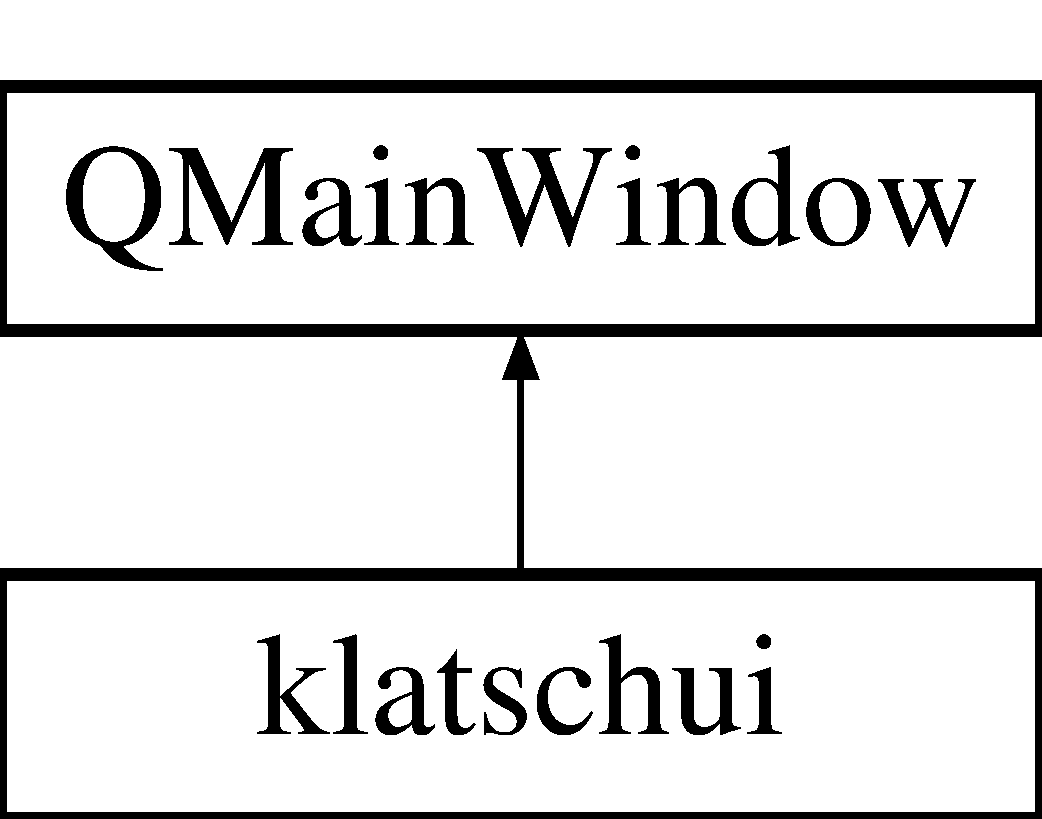
\includegraphics[height=2.000000cm]{classklatschui}
\end{center}
\end{figure}
\subsection*{Signals}
\begin{DoxyCompactItemize}
\item 
void {\bfseries write\+To\+Arduino} (Q\+String)\hypertarget{classklatschui_a2a8a15e0a55ffa93ba14b9552626b8fc}{}\label{classklatschui_a2a8a15e0a55ffa93ba14b9552626b8fc}

\item 
void {\bfseries Available\+Ports} ()\hypertarget{classklatschui_abadb649b4813dbd1fba38b4ee5014112}{}\label{classklatschui_abadb649b4813dbd1fba38b4ee5014112}

\item 
void {\bfseries Connect} (Q\+String)\hypertarget{classklatschui_a6b2513c6d27721571a2c7c599a99ce72}{}\label{classklatschui_a6b2513c6d27721571a2c7c599a99ce72}

\item 
void {\bfseries Close} ()\hypertarget{classklatschui_a91294854654b4008c24cdaa57005a7bc}{}\label{classklatschui_a91294854654b4008c24cdaa57005a7bc}

\item 
void {\bfseries clear\+Stack} ()\hypertarget{classklatschui_a667a110e7e27d635130f0253f5ffd7e7}{}\label{classklatschui_a667a110e7e27d635130f0253f5ffd7e7}

\item 
void {\bfseries fix\+Processed} ()\hypertarget{classklatschui_a744a34ae576dd7d7fdc18f87a002cf94}{}\label{classklatschui_a744a34ae576dd7d7fdc18f87a002cf94}

\end{DoxyCompactItemize}
\subsection*{Public Member Functions}
\begin{DoxyCompactItemize}
\item 
{\bfseries klatschui} (Q\+Widget $\ast$parent=0)\hypertarget{classklatschui_af0ca8331e7ccaf0b8a05bdaf6500b456}{}\label{classklatschui_af0ca8331e7ccaf0b8a05bdaf6500b456}

\end{DoxyCompactItemize}


The documentation for this class was generated from the following files\+:\begin{DoxyCompactItemize}
\item 
klatschui.\+h\item 
klatschui.\+cpp\end{DoxyCompactItemize}

\hypertarget{class_ui_1_1klatschui}{}\section{Ui\+:\+:klatschui Class Reference}
\label{class_ui_1_1klatschui}\index{Ui\+::klatschui@{Ui\+::klatschui}}
Inheritance diagram for Ui\+:\+:klatschui\+:\begin{figure}[H]
\begin{center}
\leavevmode
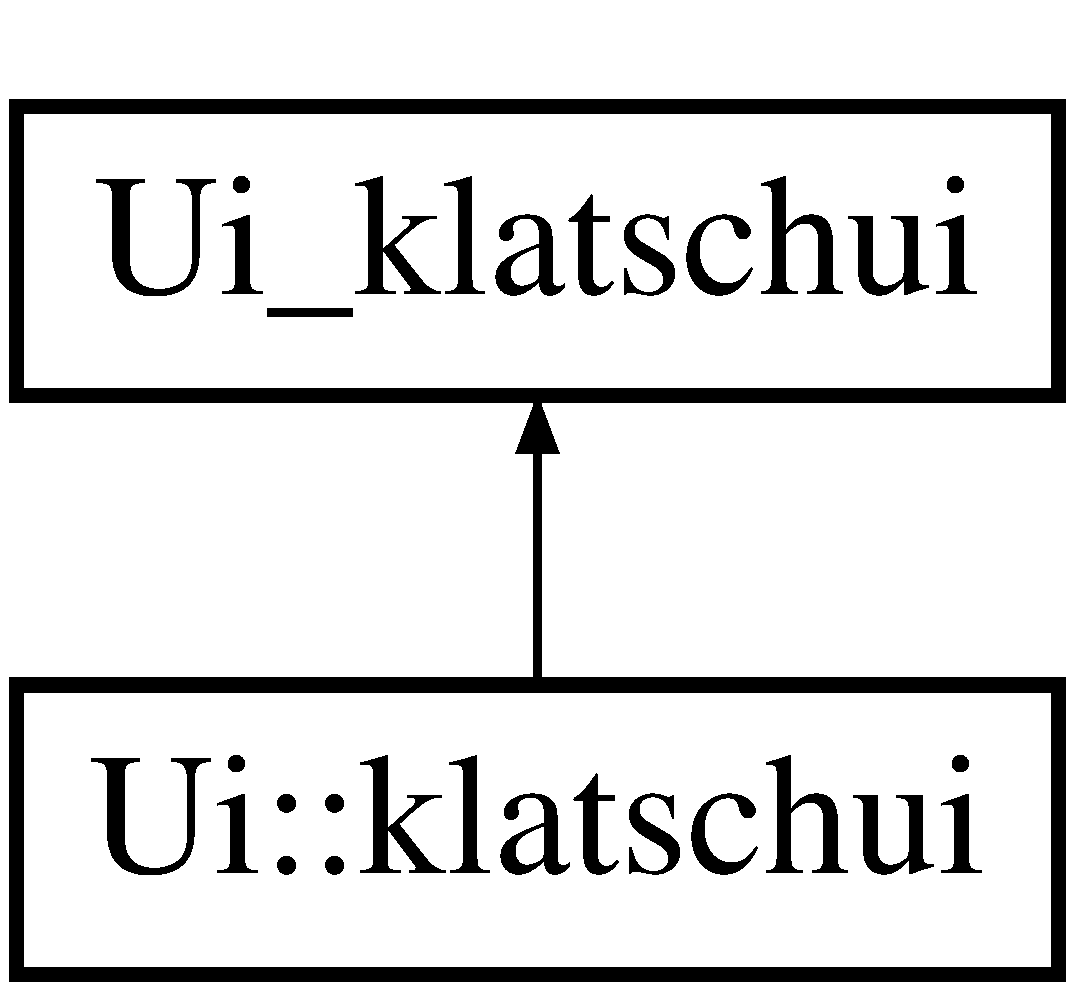
\includegraphics[height=2.000000cm]{class_ui_1_1klatschui}
\end{center}
\end{figure}
\subsection*{Additional Inherited Members}


The documentation for this class was generated from the following file\+:\begin{DoxyCompactItemize}
\item 
ui\+\_\+klatschui.\+h\end{DoxyCompactItemize}

\hypertarget{class_serial_port_listener}{}\section{Serial\+Port\+Listener Class Reference}
\label{class_serial_port_listener}\index{Serial\+Port\+Listener@{Serial\+Port\+Listener}}
Inheritance diagram for Serial\+Port\+Listener\+:\begin{figure}[H]
\begin{center}
\leavevmode
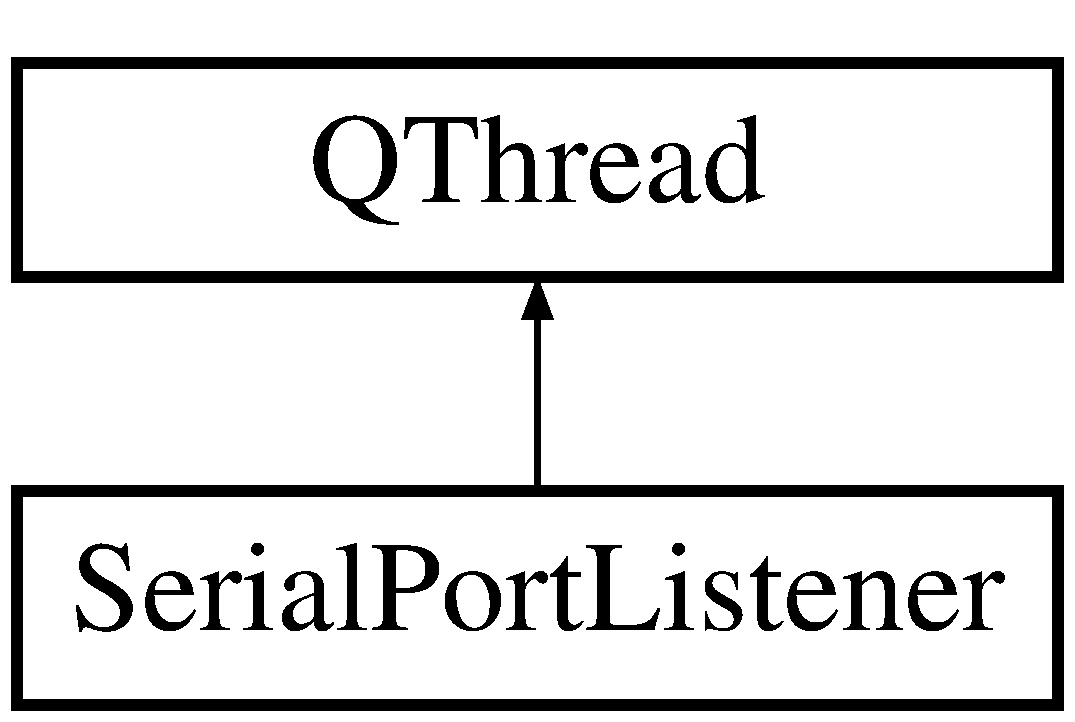
\includegraphics[height=2.000000cm]{class_serial_port_listener}
\end{center}
\end{figure}
\subsection*{Signals}
\begin{DoxyCompactItemize}
\item 
void {\bfseries data\+Received} (Q\+String)\hypertarget{class_serial_port_listener_abf1c6e95862b2d25ec0285ef77a110e9}{}\label{class_serial_port_listener_abf1c6e95862b2d25ec0285ef77a110e9}

\item 
void {\bfseries send\+Back\+Available\+Ports} (Q\+List$<$ Q\+Serial\+Port\+Info $>$, int, Q\+String)\hypertarget{class_serial_port_listener_af620ff4906c8d7653bfbd53f031896b0}{}\label{class_serial_port_listener_af620ff4906c8d7653bfbd53f031896b0}

\item 
void {\bfseries back\+To\+Connect} (int, Q\+String)\hypertarget{class_serial_port_listener_a56b44b15117baeb47509d4c0278b100e}{}\label{class_serial_port_listener_a56b44b15117baeb47509d4c0278b100e}

\item 
void {\bfseries send\+Data\+To\+Gui\+To\+Arduino} (Q\+Byte\+Array)\hypertarget{class_serial_port_listener_acc6726041672d27655578769d562acf6}{}\label{class_serial_port_listener_acc6726041672d27655578769d562acf6}

\item 
void {\bfseries number\+In\+Stack} (int)\hypertarget{class_serial_port_listener_ac5c1804cfaef3488a710044eabfbf089}{}\label{class_serial_port_listener_ac5c1804cfaef3488a710044eabfbf089}

\end{DoxyCompactItemize}
\subsection*{Public Member Functions}
\begin{DoxyCompactItemize}
\item 
{\bfseries Serial\+Port\+Listener} (Q\+Serial\+Port $\ast$serial\+Port, ulong speed)\hypertarget{class_serial_port_listener_a8a7f2051e1a51ef6a0215ed5b4bc4b6f}{}\label{class_serial_port_listener_a8a7f2051e1a51ef6a0215ed5b4bc4b6f}

\end{DoxyCompactItemize}
\subsection*{Protected Member Functions}
\begin{DoxyCompactItemize}
\item 
virtual void {\bfseries run} ()\hypertarget{class_serial_port_listener_a5dd9c170cb3c1fa515339bcecba9a692}{}\label{class_serial_port_listener_a5dd9c170cb3c1fa515339bcecba9a692}

\end{DoxyCompactItemize}


The documentation for this class was generated from the following files\+:\begin{DoxyCompactItemize}
\item 
serialportlistener.\+h\item 
serialportlistener.\+cpp\end{DoxyCompactItemize}

\hypertarget{class_ui__klatschui}{}\section{Ui\+\_\+klatschui Class Reference}
\label{class_ui__klatschui}\index{Ui\+\_\+klatschui@{Ui\+\_\+klatschui}}
Inheritance diagram for Ui\+\_\+klatschui\+:\begin{figure}[H]
\begin{center}
\leavevmode
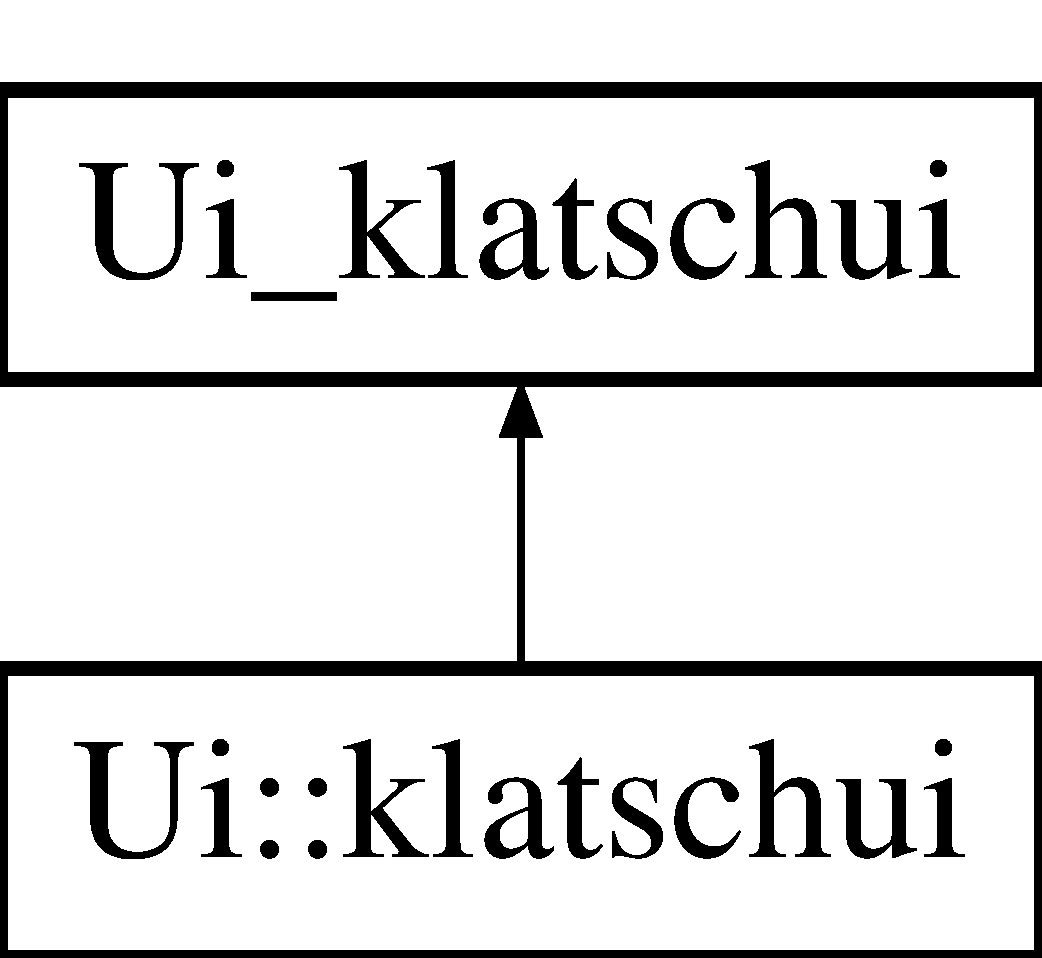
\includegraphics[height=2.000000cm]{class_ui__klatschui}
\end{center}
\end{figure}
\subsection*{Public Member Functions}
\begin{DoxyCompactItemize}
\item 
void {\bfseries setup\+Ui} (Q\+Main\+Window $\ast$\hyperlink{classklatschui}{klatschui})\hypertarget{class_ui__klatschui_a402a6ca7cea172ad1f1b037e8216b6be}{}\label{class_ui__klatschui_a402a6ca7cea172ad1f1b037e8216b6be}

\item 
void {\bfseries retranslate\+Ui} (Q\+Main\+Window $\ast$\hyperlink{classklatschui}{klatschui})\hypertarget{class_ui__klatschui_ab5513321f6e1f098260c80f6c741a925}{}\label{class_ui__klatschui_ab5513321f6e1f098260c80f6c741a925}

\end{DoxyCompactItemize}
\subsection*{Public Attributes}
\begin{DoxyCompactItemize}
\item 
Q\+Widget $\ast$ {\bfseries central\+Widget}\hypertarget{class_ui__klatschui_ae9ef1f82d80f8bcd7389d53bd4dae6e6}{}\label{class_ui__klatschui_ae9ef1f82d80f8bcd7389d53bd4dae6e6}

\item 
Q\+Tab\+Widget $\ast$ {\bfseries Tab\+Muster}\hypertarget{class_ui__klatschui_acc50b477c8c94452ee1cffc3cb9f2081}{}\label{class_ui__klatschui_acc50b477c8c94452ee1cffc3cb9f2081}

\item 
Q\+Widget $\ast$ {\bfseries Steuerung}\hypertarget{class_ui__klatschui_a6ed7fb5e0a73529113ea4cd2f6c66ead}{}\label{class_ui__klatschui_a6ed7fb5e0a73529113ea4cd2f6c66ead}

\item 
Q\+Widget $\ast$ {\bfseries layout\+Widget}\hypertarget{class_ui__klatschui_aedb29301fd0a35f323fc8e2bbe281f4b}{}\label{class_ui__klatschui_aedb29301fd0a35f323fc8e2bbe281f4b}

\item 
Q\+Grid\+Layout $\ast$ {\bfseries grid\+Layout\+\_\+7}\hypertarget{class_ui__klatschui_a00f5ffd297ca73532152341d8b002b40}{}\label{class_ui__klatschui_a00f5ffd297ca73532152341d8b002b40}

\item 
Q\+Label $\ast$ {\bfseries steu\+Ger\+Titel\+\_\+2}\hypertarget{class_ui__klatschui_a23656393e10f6e3b88ca9d09a7dd5c0d}{}\label{class_ui__klatschui_a23656393e10f6e3b88ca9d09a7dd5c0d}

\item 
Q\+Push\+Button $\ast$ {\bfseries steu\+Ger\+Aus\+\_\+20}\hypertarget{class_ui__klatschui_a165394c420fc089764f6582544865b15}{}\label{class_ui__klatschui_a165394c420fc089764f6582544865b15}

\item 
Q\+Push\+Button $\ast$ {\bfseries steu\+Ger\+Aus\+\_\+6}\hypertarget{class_ui__klatschui_a299a7cf24f987258ae0ec07864d5121e}{}\label{class_ui__klatschui_a299a7cf24f987258ae0ec07864d5121e}

\item 
Q\+Label $\ast$ {\bfseries steu\+Ger\+Titel\+\_\+10}\hypertarget{class_ui__klatschui_ae4c6eac30552aaa68ccefe076411698b}{}\label{class_ui__klatschui_ae4c6eac30552aaa68ccefe076411698b}

\item 
Q\+Label $\ast$ {\bfseries steu\+Ger\+Status\+\_\+6}\hypertarget{class_ui__klatschui_a670b046b9abbec0fce64b17f211db1be}{}\label{class_ui__klatschui_a670b046b9abbec0fce64b17f211db1be}

\item 
Q\+Push\+Button $\ast$ {\bfseries steu\+Ger\+Aus\+\_\+10}\hypertarget{class_ui__klatschui_ae112592909cd4d4166ddc8d551d0a9b3}{}\label{class_ui__klatschui_ae112592909cd4d4166ddc8d551d0a9b3}

\item 
Q\+Push\+Button $\ast$ {\bfseries steu\+Ger\+Ein\+\_\+9}\hypertarget{class_ui__klatschui_a3a5101f34be2122f2f071000b18d53e9}{}\label{class_ui__klatschui_a3a5101f34be2122f2f071000b18d53e9}

\item 
Q\+Push\+Button $\ast$ {\bfseries steu\+Ger\+Aus\+\_\+9}\hypertarget{class_ui__klatschui_a8714e821e073b5c753660299abc791ae}{}\label{class_ui__klatschui_a8714e821e073b5c753660299abc791ae}

\item 
Q\+Label $\ast$ {\bfseries steu\+Ger\+Status\+\_\+8}\hypertarget{class_ui__klatschui_a5cfbb1c4e4b8431ecdc1f2604bfd5d99}{}\label{class_ui__klatschui_a5cfbb1c4e4b8431ecdc1f2604bfd5d99}

\item 
Q\+Push\+Button $\ast$ {\bfseries steu\+Ger\+Aus\+\_\+4}\hypertarget{class_ui__klatschui_af8294f2781f349a4f9dce3c8c7d52d9f}{}\label{class_ui__klatschui_af8294f2781f349a4f9dce3c8c7d52d9f}

\item 
Q\+Push\+Button $\ast$ {\bfseries steu\+Ger\+Ein\+\_\+21}\hypertarget{class_ui__klatschui_a156ec155050d1953e214e893e0d99cfd}{}\label{class_ui__klatschui_a156ec155050d1953e214e893e0d99cfd}

\item 
Q\+Push\+Button $\ast$ {\bfseries steu\+Ger\+Aus\+\_\+7}\hypertarget{class_ui__klatschui_ad0de78934769b8415a89aeb607aa18d4}{}\label{class_ui__klatschui_ad0de78934769b8415a89aeb607aa18d4}

\item 
Q\+Label $\ast$ {\bfseries steu\+Ger\+Titel\+\_\+7}\hypertarget{class_ui__klatschui_ac562466f72cc85910f21424bf26a5d58}{}\label{class_ui__klatschui_ac562466f72cc85910f21424bf26a5d58}

\item 
Q\+Label $\ast$ {\bfseries steu\+Ger\+Titel\+\_\+0}\hypertarget{class_ui__klatschui_aa62c01980fc731aa28f284eb58243387}{}\label{class_ui__klatschui_aa62c01980fc731aa28f284eb58243387}

\item 
Q\+Label $\ast$ {\bfseries steu\+Ger\+Status\+\_\+21}\hypertarget{class_ui__klatschui_a15acb16ac1cf14dded4ac891000b9a88}{}\label{class_ui__klatschui_a15acb16ac1cf14dded4ac891000b9a88}

\item 
Q\+Label $\ast$ {\bfseries steu\+Ger\+Titel\+\_\+5}\hypertarget{class_ui__klatschui_a236b5b7d5e4ae694f24017b52c352135}{}\label{class_ui__klatschui_a236b5b7d5e4ae694f24017b52c352135}

\item 
Q\+Label $\ast$ {\bfseries steu\+Ger\+Status\+\_\+10}\hypertarget{class_ui__klatschui_a11367f4653626999588f0d48d10a8298}{}\label{class_ui__klatschui_a11367f4653626999588f0d48d10a8298}

\item 
Q\+Label $\ast$ {\bfseries steu\+Ger\+Status\+\_\+5}\hypertarget{class_ui__klatschui_a6b529f0e69104597ba40e147ab311c05}{}\label{class_ui__klatschui_a6b529f0e69104597ba40e147ab311c05}

\item 
Q\+Push\+Button $\ast$ {\bfseries steu\+Ger\+Ein\+\_\+4}\hypertarget{class_ui__klatschui_a847864748df26a38f3fff003bced8443}{}\label{class_ui__klatschui_a847864748df26a38f3fff003bced8443}

\item 
Q\+Label $\ast$ {\bfseries steu\+Ger\+Titel\+\_\+8}\hypertarget{class_ui__klatschui_a18bd56de5636df39c6d381e290c83f6c}{}\label{class_ui__klatschui_a18bd56de5636df39c6d381e290c83f6c}

\item 
Q\+Label $\ast$ {\bfseries steu\+Ger\+Status\+\_\+9}\hypertarget{class_ui__klatschui_a124feea81f4c25315e97c882f3d2c660}{}\label{class_ui__klatschui_a124feea81f4c25315e97c882f3d2c660}

\item 
Q\+Label $\ast$ {\bfseries steu\+Ger\+Titel\+\_\+3}\hypertarget{class_ui__klatschui_a79855bdcfaa5606f496e5a81cad73e66}{}\label{class_ui__klatschui_a79855bdcfaa5606f496e5a81cad73e66}

\item 
Q\+Push\+Button $\ast$ {\bfseries steu\+Ger\+Ein\+\_\+20}\hypertarget{class_ui__klatschui_a296bc25c6d22d502b3efe9b7df28834e}{}\label{class_ui__klatschui_a296bc25c6d22d502b3efe9b7df28834e}

\item 
Q\+Label $\ast$ {\bfseries steu\+Ger\+Status\+\_\+4}\hypertarget{class_ui__klatschui_a7212b1054221cd704ee93247959c1500}{}\label{class_ui__klatschui_a7212b1054221cd704ee93247959c1500}

\item 
Q\+Label $\ast$ {\bfseries steu\+Ger\+Status\+\_\+7}\hypertarget{class_ui__klatschui_a7b936831a4b12f561092ee06749c2075}{}\label{class_ui__klatschui_a7b936831a4b12f561092ee06749c2075}

\item 
Q\+Push\+Button $\ast$ {\bfseries steu\+Ger\+Aus\+\_\+5}\hypertarget{class_ui__klatschui_a22d5fa25ddefa19bd1c89a109741c744}{}\label{class_ui__klatschui_a22d5fa25ddefa19bd1c89a109741c744}

\item 
Q\+Push\+Button $\ast$ {\bfseries steu\+Ger\+Ein\+\_\+10}\hypertarget{class_ui__klatschui_ad5bb165eb6c5e997acc519cee465127e}{}\label{class_ui__klatschui_ad5bb165eb6c5e997acc519cee465127e}

\item 
Q\+Push\+Button $\ast$ {\bfseries steu\+Ger\+Ein\+\_\+7}\hypertarget{class_ui__klatschui_ae25d93b22b7d0003e498416d1a5b290b}{}\label{class_ui__klatschui_ae25d93b22b7d0003e498416d1a5b290b}

\item 
Q\+Push\+Button $\ast$ {\bfseries steu\+Ger\+Ein\+\_\+6}\hypertarget{class_ui__klatschui_a4f47b5524d0579bd6b44ec19ad526d02}{}\label{class_ui__klatschui_a4f47b5524d0579bd6b44ec19ad526d02}

\item 
Q\+Label $\ast$ {\bfseries steu\+Ger\+Titel\+\_\+6}\hypertarget{class_ui__klatschui_ada1ae1fd2be2c8252692bed0ee6354a5}{}\label{class_ui__klatschui_ada1ae1fd2be2c8252692bed0ee6354a5}

\item 
Q\+Label $\ast$ {\bfseries steu\+Ger\+Status\+\_\+20}\hypertarget{class_ui__klatschui_aac6c79428351aef3ac570b6770741d31}{}\label{class_ui__klatschui_aac6c79428351aef3ac570b6770741d31}

\item 
Q\+Label $\ast$ {\bfseries steu\+Ger\+Titel\+\_\+9}\hypertarget{class_ui__klatschui_a5c05558764bd37267b38c9575901ba7b}{}\label{class_ui__klatschui_a5c05558764bd37267b38c9575901ba7b}

\item 
Q\+Label $\ast$ {\bfseries steu\+Ger\+Titel\+\_\+21}\hypertarget{class_ui__klatschui_a7d546ebaa5e20c5dd8250b8c5dad1720}{}\label{class_ui__klatschui_a7d546ebaa5e20c5dd8250b8c5dad1720}

\item 
Q\+Push\+Button $\ast$ {\bfseries steu\+Ger\+Ein\+\_\+5}\hypertarget{class_ui__klatschui_ae3b1b3eccecee61f39fdb56fae0ed7a3}{}\label{class_ui__klatschui_ae3b1b3eccecee61f39fdb56fae0ed7a3}

\item 
Q\+Push\+Button $\ast$ {\bfseries steu\+Ger\+Ein\+\_\+2}\hypertarget{class_ui__klatschui_a4a2efcb70b71144aebae15d98274ec32}{}\label{class_ui__klatschui_a4a2efcb70b71144aebae15d98274ec32}

\item 
Q\+Push\+Button $\ast$ {\bfseries steu\+Ger\+Aus\+\_\+21}\hypertarget{class_ui__klatschui_ac2d2ac0ac8e20d94b60ac875292e462b}{}\label{class_ui__klatschui_ac2d2ac0ac8e20d94b60ac875292e462b}

\item 
Q\+Push\+Button $\ast$ {\bfseries steu\+Ger\+Aus\+\_\+2}\hypertarget{class_ui__klatschui_a051f7cb4a7d35adf37b09915ef087a7b}{}\label{class_ui__klatschui_a051f7cb4a7d35adf37b09915ef087a7b}

\item 
Q\+Push\+Button $\ast$ {\bfseries steu\+Ger\+Ein\+\_\+8}\hypertarget{class_ui__klatschui_a99d782e1d99fdb77921b74805afc3ca9}{}\label{class_ui__klatschui_a99d782e1d99fdb77921b74805afc3ca9}

\item 
Q\+Label $\ast$ {\bfseries steu\+Ger\+Titel\+\_\+20}\hypertarget{class_ui__klatschui_a39e312920658012fe2d91080ab4f07ad}{}\label{class_ui__klatschui_a39e312920658012fe2d91080ab4f07ad}

\item 
Q\+Push\+Button $\ast$ {\bfseries steu\+Ger\+Aus\+\_\+8}\hypertarget{class_ui__klatschui_ab12bb0b93bb92f187f9be706ed23d59f}{}\label{class_ui__klatschui_ab12bb0b93bb92f187f9be706ed23d59f}

\item 
Q\+Label $\ast$ {\bfseries steu\+Ger\+Status\+\_\+2}\hypertarget{class_ui__klatschui_af6c6156826ebd4b3a4d782f4a6cb99a8}{}\label{class_ui__klatschui_af6c6156826ebd4b3a4d782f4a6cb99a8}

\item 
Q\+Push\+Button $\ast$ {\bfseries steu\+Ger\+Ein\+\_\+0}\hypertarget{class_ui__klatschui_a022108d4c8d4e7a762548e20bdc7506d}{}\label{class_ui__klatschui_a022108d4c8d4e7a762548e20bdc7506d}

\item 
Q\+Push\+Button $\ast$ {\bfseries steu\+Ger\+Aus\+\_\+0}\hypertarget{class_ui__klatschui_abb8bfa7456d97c00104c677a19e8ba73}{}\label{class_ui__klatschui_abb8bfa7456d97c00104c677a19e8ba73}

\item 
Q\+Label $\ast$ {\bfseries steu\+Ger\+Status\+\_\+0}\hypertarget{class_ui__klatschui_a85a95dadf6b8eab3ba23c42067bcc240}{}\label{class_ui__klatschui_a85a95dadf6b8eab3ba23c42067bcc240}

\item 
Q\+Widget $\ast$ {\bfseries tab\+Muster}\hypertarget{class_ui__klatschui_a2920e45cf75ef94c4db381ed7802a58d}{}\label{class_ui__klatschui_a2920e45cf75ef94c4db381ed7802a58d}

\item 
Q\+Widget $\ast$ {\bfseries layout\+Widget1}\hypertarget{class_ui__klatschui_ab1030e7cff7271caec68a37e6ab20015}{}\label{class_ui__klatschui_ab1030e7cff7271caec68a37e6ab20015}

\item 
Q\+Grid\+Layout $\ast$ {\bfseries grid\+Layout\+\_\+8}\hypertarget{class_ui__klatschui_a35745d73946f69748cce2b5459fb081c}{}\label{class_ui__klatschui_a35745d73946f69748cce2b5459fb081c}

\item 
Q\+Push\+Button $\ast$ {\bfseries mus\+Save}\hypertarget{class_ui__klatschui_ae2f9e0746b520d5473e6980899f095f5}{}\label{class_ui__klatschui_ae2f9e0746b520d5473e6980899f095f5}

\item 
Q\+Combo\+Box $\ast$ {\bfseries mus\+Action\+\_\+10}\hypertarget{class_ui__klatschui_ab723220f5b24e38239880eec4b0ab4cc}{}\label{class_ui__klatschui_ab723220f5b24e38239880eec4b0ab4cc}

\item 
Q\+Push\+Button $\ast$ {\bfseries mus\+Clear}\hypertarget{class_ui__klatschui_a7dc315ff74314e62e9cd66893a47dfc6}{}\label{class_ui__klatschui_a7dc315ff74314e62e9cd66893a47dfc6}

\item 
Q\+Line\+Edit $\ast$ {\bfseries mus\+Ger\+\_\+10}\hypertarget{class_ui__klatschui_ab18e2b0df6bd04913abb0cc7adc9945b}{}\label{class_ui__klatschui_ab18e2b0df6bd04913abb0cc7adc9945b}

\item 
Q\+Push\+Button $\ast$ {\bfseries mus\+Save\+\_\+10}\hypertarget{class_ui__klatschui_a184f5a7741d6e33339698475669d981d}{}\label{class_ui__klatschui_a184f5a7741d6e33339698475669d981d}

\item 
Q\+Combo\+Box $\ast$ {\bfseries mus10m4}\hypertarget{class_ui__klatschui_a6babf1274b0a95ae2d4ed193bc608575}{}\label{class_ui__klatschui_a6babf1274b0a95ae2d4ed193bc608575}

\item 
Q\+Combo\+Box $\ast$ {\bfseries mus10m5}\hypertarget{class_ui__klatschui_abf6f4a3a920d0912012e1896a05eab38}{}\label{class_ui__klatschui_abf6f4a3a920d0912012e1896a05eab38}

\item 
Q\+Combo\+Box $\ast$ {\bfseries mus10m1}\hypertarget{class_ui__klatschui_a6c47e9a81051d1a2870348a3f5e2939d}{}\label{class_ui__klatschui_a6c47e9a81051d1a2870348a3f5e2939d}

\item 
Q\+Combo\+Box $\ast$ {\bfseries mus10m2}\hypertarget{class_ui__klatschui_aed7bef89e25cc07ef6fee211faee4d33}{}\label{class_ui__klatschui_aed7bef89e25cc07ef6fee211faee4d33}

\item 
Q\+Combo\+Box $\ast$ {\bfseries mus10m3}\hypertarget{class_ui__klatschui_a923e271fe346a7cb6f490b37e092e713}{}\label{class_ui__klatschui_a923e271fe346a7cb6f490b37e092e713}

\item 
Q\+Line\+Edit $\ast$ {\bfseries mus\+Line\+\_\+10}\hypertarget{class_ui__klatschui_ac8ec3428c674a41bdf78306a454f3555}{}\label{class_ui__klatschui_ac8ec3428c674a41bdf78306a454f3555}

\item 
Q\+Label $\ast$ {\bfseries mus\+Lab10}\hypertarget{class_ui__klatschui_a1376c8da4705e8e477c6b699f4a59f90}{}\label{class_ui__klatschui_a1376c8da4705e8e477c6b699f4a59f90}

\item 
Q\+Push\+Button $\ast$ {\bfseries mus\+Save\+\_\+9}\hypertarget{class_ui__klatschui_a9c8fb2d220d0a028d25abdd758e0c269}{}\label{class_ui__klatschui_a9c8fb2d220d0a028d25abdd758e0c269}

\item 
Q\+Combo\+Box $\ast$ {\bfseries mus\+Action\+\_\+9}\hypertarget{class_ui__klatschui_a6d1effa45fa56d237b8aa9aa0545c577}{}\label{class_ui__klatschui_a6d1effa45fa56d237b8aa9aa0545c577}

\item 
Q\+Line\+Edit $\ast$ {\bfseries mus\+Ger\+\_\+9}\hypertarget{class_ui__klatschui_a64b3223cd7118e32daec75f4c71d038c}{}\label{class_ui__klatschui_a64b3223cd7118e32daec75f4c71d038c}

\item 
Q\+Combo\+Box $\ast$ {\bfseries mus9m4}\hypertarget{class_ui__klatschui_abae71350442d6b1b7b9347648fbd438d}{}\label{class_ui__klatschui_abae71350442d6b1b7b9347648fbd438d}

\item 
Q\+Combo\+Box $\ast$ {\bfseries mus9m5}\hypertarget{class_ui__klatschui_a3cbf286064bcfd42645d2a3fb6d28fa4}{}\label{class_ui__klatschui_a3cbf286064bcfd42645d2a3fb6d28fa4}

\item 
Q\+Combo\+Box $\ast$ {\bfseries mus9m3}\hypertarget{class_ui__klatschui_ab60b7969821f8f45a0680ef5d7d0fc62}{}\label{class_ui__klatschui_ab60b7969821f8f45a0680ef5d7d0fc62}

\item 
Q\+Combo\+Box $\ast$ {\bfseries mus9m1}\hypertarget{class_ui__klatschui_a3694949d8f16a7df3c0278c3b79484d9}{}\label{class_ui__klatschui_a3694949d8f16a7df3c0278c3b79484d9}

\item 
Q\+Line\+Edit $\ast$ {\bfseries mus\+Line\+\_\+9}\hypertarget{class_ui__klatschui_a0dec9a936aeb05c4b71d1143aa00859d}{}\label{class_ui__klatschui_a0dec9a936aeb05c4b71d1143aa00859d}

\item 
Q\+Combo\+Box $\ast$ {\bfseries mus9m2}\hypertarget{class_ui__klatschui_a043ef81b1613907757e6ca652f00acfb}{}\label{class_ui__klatschui_a043ef81b1613907757e6ca652f00acfb}

\item 
Q\+Label $\ast$ {\bfseries mus\+Lab9}\hypertarget{class_ui__klatschui_a7ffeda19fbddd56b1dac38050b1b0147}{}\label{class_ui__klatschui_a7ffeda19fbddd56b1dac38050b1b0147}

\item 
Q\+Line\+Edit $\ast$ {\bfseries mus\+Ger\+\_\+8}\hypertarget{class_ui__klatschui_a8ebc7f90a57179288155351fbba6da9b}{}\label{class_ui__klatschui_a8ebc7f90a57179288155351fbba6da9b}

\item 
Q\+Push\+Button $\ast$ {\bfseries mus\+Save\+\_\+8}\hypertarget{class_ui__klatschui_a5be2627bf48fdbcd5985e6b95a2440f4}{}\label{class_ui__klatschui_a5be2627bf48fdbcd5985e6b95a2440f4}

\item 
Q\+Combo\+Box $\ast$ {\bfseries mus\+Action\+\_\+8}\hypertarget{class_ui__klatschui_a36b376e7aec4652395c4d24c05d1441b}{}\label{class_ui__klatschui_a36b376e7aec4652395c4d24c05d1441b}

\item 
Q\+Combo\+Box $\ast$ {\bfseries mus8m5}\hypertarget{class_ui__klatschui_ad6e4d97f21cf068b361850a2fc47945c}{}\label{class_ui__klatschui_ad6e4d97f21cf068b361850a2fc47945c}

\item 
Q\+Combo\+Box $\ast$ {\bfseries mus8m3}\hypertarget{class_ui__klatschui_a936ab4b2c046227295d758f5ecd3aba4}{}\label{class_ui__klatschui_a936ab4b2c046227295d758f5ecd3aba4}

\item 
Q\+Combo\+Box $\ast$ {\bfseries mus8m4}\hypertarget{class_ui__klatschui_a9cc3fa0e0c23a9070390358ca0482703}{}\label{class_ui__klatschui_a9cc3fa0e0c23a9070390358ca0482703}

\item 
Q\+Combo\+Box $\ast$ {\bfseries mus8m2}\hypertarget{class_ui__klatschui_a44d44c047778721aea75eec5122e4309}{}\label{class_ui__klatschui_a44d44c047778721aea75eec5122e4309}

\item 
Q\+Combo\+Box $\ast$ {\bfseries mus8m1}\hypertarget{class_ui__klatschui_a58369c605340deccb4781cfa93aa8e27}{}\label{class_ui__klatschui_a58369c605340deccb4781cfa93aa8e27}

\item 
Q\+Label $\ast$ {\bfseries mus\+Lab8}\hypertarget{class_ui__klatschui_ae5e989147baf6f52b5ce3ef3604a1b63}{}\label{class_ui__klatschui_ae5e989147baf6f52b5ce3ef3604a1b63}

\item 
Q\+Line\+Edit $\ast$ {\bfseries mus\+Line\+\_\+8}\hypertarget{class_ui__klatschui_afe99f59ac28a731ca752e70197709437}{}\label{class_ui__klatschui_afe99f59ac28a731ca752e70197709437}

\item 
Q\+Push\+Button $\ast$ {\bfseries mus\+Save\+\_\+7}\hypertarget{class_ui__klatschui_ad86fb8d3a0d81cac1a643986d5af7f17}{}\label{class_ui__klatschui_ad86fb8d3a0d81cac1a643986d5af7f17}

\item 
Q\+Combo\+Box $\ast$ {\bfseries mus\+Action\+\_\+7}\hypertarget{class_ui__klatschui_a7f474ebad9847cceb83bfa2dfb57ea85}{}\label{class_ui__klatschui_a7f474ebad9847cceb83bfa2dfb57ea85}

\item 
Q\+Line\+Edit $\ast$ {\bfseries mus\+Ger\+\_\+7}\hypertarget{class_ui__klatschui_a8cc36d684eff9a5d04d69ac5783e12f0}{}\label{class_ui__klatschui_a8cc36d684eff9a5d04d69ac5783e12f0}

\item 
Q\+Combo\+Box $\ast$ {\bfseries mus7m5}\hypertarget{class_ui__klatschui_a41ccd93c99648230469565e599b1cff8}{}\label{class_ui__klatschui_a41ccd93c99648230469565e599b1cff8}

\item 
Q\+Combo\+Box $\ast$ {\bfseries mus7m4}\hypertarget{class_ui__klatschui_acc3535261b89af1df822554b393445ad}{}\label{class_ui__klatschui_acc3535261b89af1df822554b393445ad}

\item 
Q\+Combo\+Box $\ast$ {\bfseries mus7m2}\hypertarget{class_ui__klatschui_a87151c3c336323944afbb5c7fa457a6c}{}\label{class_ui__klatschui_a87151c3c336323944afbb5c7fa457a6c}

\item 
Q\+Combo\+Box $\ast$ {\bfseries mus7m3}\hypertarget{class_ui__klatschui_a22b74ce664960b446bf30acd4bbf110d}{}\label{class_ui__klatschui_a22b74ce664960b446bf30acd4bbf110d}

\item 
Q\+Line\+Edit $\ast$ {\bfseries mus\+Line\+\_\+7}\hypertarget{class_ui__klatschui_acb8487308fb0b8414152cd2bbb88ae5e}{}\label{class_ui__klatschui_acb8487308fb0b8414152cd2bbb88ae5e}

\item 
Q\+Combo\+Box $\ast$ {\bfseries mus7m1}\hypertarget{class_ui__klatschui_a8199ccf559cba6713cc06fe5fcea638d}{}\label{class_ui__klatschui_a8199ccf559cba6713cc06fe5fcea638d}

\item 
Q\+Label $\ast$ {\bfseries mus\+Lab7}\hypertarget{class_ui__klatschui_a6b7ad8db719d2ed195d5d5c639676de1}{}\label{class_ui__klatschui_a6b7ad8db719d2ed195d5d5c639676de1}

\item 
Q\+Push\+Button $\ast$ {\bfseries mus\+Save\+\_\+6}\hypertarget{class_ui__klatschui_af6dbd408dd81fc42f5112121215e20ef}{}\label{class_ui__klatschui_af6dbd408dd81fc42f5112121215e20ef}

\item 
Q\+Combo\+Box $\ast$ {\bfseries mus\+Action\+\_\+6}\hypertarget{class_ui__klatschui_a6037d66b1a72a7c427e13ad7df45d9c1}{}\label{class_ui__klatschui_a6037d66b1a72a7c427e13ad7df45d9c1}

\item 
Q\+Line\+Edit $\ast$ {\bfseries mus\+Ger\+\_\+6}\hypertarget{class_ui__klatschui_a4cd9352b26a9fb8349ce433442d03db1}{}\label{class_ui__klatschui_a4cd9352b26a9fb8349ce433442d03db1}

\item 
Q\+Combo\+Box $\ast$ {\bfseries mus6m4}\hypertarget{class_ui__klatschui_a12801232bb020b6fc7c420cafed3cdc9}{}\label{class_ui__klatschui_a12801232bb020b6fc7c420cafed3cdc9}

\item 
Q\+Combo\+Box $\ast$ {\bfseries mus6m2}\hypertarget{class_ui__klatschui_acc8665d926a26f919a9cccbfc4732fce}{}\label{class_ui__klatschui_acc8665d926a26f919a9cccbfc4732fce}

\item 
Q\+Combo\+Box $\ast$ {\bfseries mus6m5}\hypertarget{class_ui__klatschui_af7240380802e0de6151a03fbe4ea9f84}{}\label{class_ui__klatschui_af7240380802e0de6151a03fbe4ea9f84}

\item 
Q\+Combo\+Box $\ast$ {\bfseries mus6m3}\hypertarget{class_ui__klatschui_aa392919e95a3f0bcb67b6bede3919671}{}\label{class_ui__klatschui_aa392919e95a3f0bcb67b6bede3919671}

\item 
Q\+Line\+Edit $\ast$ {\bfseries mus\+Line\+\_\+6}\hypertarget{class_ui__klatschui_af41b5f63c4d8a029a02fbba6a165500f}{}\label{class_ui__klatschui_af41b5f63c4d8a029a02fbba6a165500f}

\item 
Q\+Combo\+Box $\ast$ {\bfseries mus6m1}\hypertarget{class_ui__klatschui_a2385f00c5cd7eb11a87c0a27ac0bcd68}{}\label{class_ui__klatschui_a2385f00c5cd7eb11a87c0a27ac0bcd68}

\item 
Q\+Label $\ast$ {\bfseries mus\+Lab6}\hypertarget{class_ui__klatschui_ac45896a0ce7718241b39321489410193}{}\label{class_ui__klatschui_ac45896a0ce7718241b39321489410193}

\item 
Q\+Push\+Button $\ast$ {\bfseries mus\+Save\+\_\+5}\hypertarget{class_ui__klatschui_a11d398a60579e9af593a2db542e680b8}{}\label{class_ui__klatschui_a11d398a60579e9af593a2db542e680b8}

\item 
Q\+Line\+Edit $\ast$ {\bfseries mus\+Ger\+\_\+5}\hypertarget{class_ui__klatschui_af60eeb3be940d3e30e76616ae37b05c8}{}\label{class_ui__klatschui_af60eeb3be940d3e30e76616ae37b05c8}

\item 
Q\+Combo\+Box $\ast$ {\bfseries mus\+Action\+\_\+5}\hypertarget{class_ui__klatschui_aad3985e34447f19a2d34917674e6b085}{}\label{class_ui__klatschui_aad3985e34447f19a2d34917674e6b085}

\item 
Q\+Combo\+Box $\ast$ {\bfseries mus5m4}\hypertarget{class_ui__klatschui_a9ddc4a7c855383ec07d6035dc4f015f3}{}\label{class_ui__klatschui_a9ddc4a7c855383ec07d6035dc4f015f3}

\item 
Q\+Combo\+Box $\ast$ {\bfseries mus5m2}\hypertarget{class_ui__klatschui_ada7262e69c224c4c704b17fa8d292797}{}\label{class_ui__klatschui_ada7262e69c224c4c704b17fa8d292797}

\item 
Q\+Combo\+Box $\ast$ {\bfseries mus5m5}\hypertarget{class_ui__klatschui_a5c464df861e5b35991bf158a62df15af}{}\label{class_ui__klatschui_a5c464df861e5b35991bf158a62df15af}

\item 
Q\+Combo\+Box $\ast$ {\bfseries mus5m3}\hypertarget{class_ui__klatschui_aece8dd4eec015a53cb477b0ac31aa803}{}\label{class_ui__klatschui_aece8dd4eec015a53cb477b0ac31aa803}

\item 
Q\+Line\+Edit $\ast$ {\bfseries mus\+Line\+\_\+5}\hypertarget{class_ui__klatschui_aa67773c6c587a2d8f4349d2ec8c8aa6f}{}\label{class_ui__klatschui_aa67773c6c587a2d8f4349d2ec8c8aa6f}

\item 
Q\+Push\+Button $\ast$ {\bfseries mus\+Save\+\_\+4}\hypertarget{class_ui__klatschui_aa4f9b99ea224c70e37838f1bd6899a2a}{}\label{class_ui__klatschui_aa4f9b99ea224c70e37838f1bd6899a2a}

\item 
Q\+Label $\ast$ {\bfseries mus\+Lab5}\hypertarget{class_ui__klatschui_a1b115eaf74bc4b443aec994411790bd2}{}\label{class_ui__klatschui_a1b115eaf74bc4b443aec994411790bd2}

\item 
Q\+Combo\+Box $\ast$ {\bfseries mus5m1}\hypertarget{class_ui__klatschui_a7574c5a5be3dc221ccb94c7862042bd6}{}\label{class_ui__klatschui_a7574c5a5be3dc221ccb94c7862042bd6}

\item 
Q\+Combo\+Box $\ast$ {\bfseries mus\+Action\+\_\+4}\hypertarget{class_ui__klatschui_acfb0088be984a5574dd6a640886a9721}{}\label{class_ui__klatschui_acfb0088be984a5574dd6a640886a9721}

\item 
Q\+Combo\+Box $\ast$ {\bfseries mus4m5}\hypertarget{class_ui__klatschui_a907dc30893594b1a0765fee0970fdca6}{}\label{class_ui__klatschui_a907dc30893594b1a0765fee0970fdca6}

\item 
Q\+Line\+Edit $\ast$ {\bfseries mus\+Ger\+\_\+4}\hypertarget{class_ui__klatschui_a0530a82b178fb4d6fd04a17a7ab3f729}{}\label{class_ui__klatschui_a0530a82b178fb4d6fd04a17a7ab3f729}

\item 
Q\+Combo\+Box $\ast$ {\bfseries mus4m4}\hypertarget{class_ui__klatschui_a40aa1ca8103ab6b635be8f847adde09a}{}\label{class_ui__klatschui_a40aa1ca8103ab6b635be8f847adde09a}

\item 
Q\+Combo\+Box $\ast$ {\bfseries mus4m2}\hypertarget{class_ui__klatschui_a930c3d45d8d62598b017dbc27431e9d8}{}\label{class_ui__klatschui_a930c3d45d8d62598b017dbc27431e9d8}

\item 
Q\+Line\+Edit $\ast$ {\bfseries mus\+Line\+\_\+4}\hypertarget{class_ui__klatschui_a1603890e5b6e65c164ff15550b446f2e}{}\label{class_ui__klatschui_a1603890e5b6e65c164ff15550b446f2e}

\item 
Q\+Combo\+Box $\ast$ {\bfseries mus4m3}\hypertarget{class_ui__klatschui_a410e273384958bb40c15e84030a93d19}{}\label{class_ui__klatschui_a410e273384958bb40c15e84030a93d19}

\item 
Q\+Label $\ast$ {\bfseries mus\+Lab4}\hypertarget{class_ui__klatschui_a422bfb591655750224eac121bb8d2664}{}\label{class_ui__klatschui_a422bfb591655750224eac121bb8d2664}

\item 
Q\+Combo\+Box $\ast$ {\bfseries mus4m1}\hypertarget{class_ui__klatschui_a2b4110485069bae078df1be8165e79a7}{}\label{class_ui__klatschui_a2b4110485069bae078df1be8165e79a7}

\item 
Q\+Push\+Button $\ast$ {\bfseries mus\+Save\+\_\+3}\hypertarget{class_ui__klatschui_a62204f6e36ab62b71556d1ff4396a346}{}\label{class_ui__klatschui_a62204f6e36ab62b71556d1ff4396a346}

\item 
Q\+Combo\+Box $\ast$ {\bfseries mus\+Action\+\_\+3}\hypertarget{class_ui__klatschui_a805e023b3907c19aa28a9be627d36079}{}\label{class_ui__klatschui_a805e023b3907c19aa28a9be627d36079}

\item 
Q\+Line\+Edit $\ast$ {\bfseries mus\+Ger\+\_\+3}\hypertarget{class_ui__klatschui_ab82f6ef16b86c59ffacdc751292e26c0}{}\label{class_ui__klatschui_ab82f6ef16b86c59ffacdc751292e26c0}

\item 
Q\+Combo\+Box $\ast$ {\bfseries mus3m4}\hypertarget{class_ui__klatschui_a3bd9c6f3aed96b10bb2ae3b42f0332f1}{}\label{class_ui__klatschui_a3bd9c6f3aed96b10bb2ae3b42f0332f1}

\item 
Q\+Combo\+Box $\ast$ {\bfseries mus3m3}\hypertarget{class_ui__klatschui_ab339fd297e73a242f231af30fc5fc7d4}{}\label{class_ui__klatschui_ab339fd297e73a242f231af30fc5fc7d4}

\item 
Q\+Combo\+Box $\ast$ {\bfseries mus3m5}\hypertarget{class_ui__klatschui_acc0ce8ba6567ac0d362eca4fb8f04473}{}\label{class_ui__klatschui_acc0ce8ba6567ac0d362eca4fb8f04473}

\item 
Q\+Combo\+Box $\ast$ {\bfseries mus3m2}\hypertarget{class_ui__klatschui_a1fa138107b44b0ce8076ae7aa665b573}{}\label{class_ui__klatschui_a1fa138107b44b0ce8076ae7aa665b573}

\item 
Q\+Combo\+Box $\ast$ {\bfseries mus3m1}\hypertarget{class_ui__klatschui_a60283aad5206db609ed3fc84a9f3280a}{}\label{class_ui__klatschui_a60283aad5206db609ed3fc84a9f3280a}

\item 
Q\+Line\+Edit $\ast$ {\bfseries mus\+Line\+\_\+3}\hypertarget{class_ui__klatschui_a2966ed561c732118d23ab19e3d9e58ba}{}\label{class_ui__klatschui_a2966ed561c732118d23ab19e3d9e58ba}

\item 
Q\+Label $\ast$ {\bfseries mus\+Lab3}\hypertarget{class_ui__klatschui_a826d9a913c44550f2389c152487244a4}{}\label{class_ui__klatschui_a826d9a913c44550f2389c152487244a4}

\item 
Q\+Combo\+Box $\ast$ {\bfseries mus\+Action\+\_\+2}\hypertarget{class_ui__klatschui_a38394cff9b5960e764229b33cd7a72aa}{}\label{class_ui__klatschui_a38394cff9b5960e764229b33cd7a72aa}

\item 
Q\+Push\+Button $\ast$ {\bfseries mus\+Save\+\_\+2}\hypertarget{class_ui__klatschui_a4bb60b4694ddbcbee714ce2273989861}{}\label{class_ui__klatschui_a4bb60b4694ddbcbee714ce2273989861}

\item 
Q\+Line\+Edit $\ast$ {\bfseries mus\+Ger\+\_\+2}\hypertarget{class_ui__klatschui_afb19168518463b6a158170c64d60a0a6}{}\label{class_ui__klatschui_afb19168518463b6a158170c64d60a0a6}

\item 
Q\+Combo\+Box $\ast$ {\bfseries mus2m4}\hypertarget{class_ui__klatschui_a224ce8d21d9e3be50fdb3deeaec83bd5}{}\label{class_ui__klatschui_a224ce8d21d9e3be50fdb3deeaec83bd5}

\item 
Q\+Combo\+Box $\ast$ {\bfseries mus2m3}\hypertarget{class_ui__klatschui_a3d0f732d60db33eb368085bf6d43f95c}{}\label{class_ui__klatschui_a3d0f732d60db33eb368085bf6d43f95c}

\item 
Q\+Combo\+Box $\ast$ {\bfseries mus2m5}\hypertarget{class_ui__klatschui_aeb7a0c8bed60fecbc9087f1e09d5c72a}{}\label{class_ui__klatschui_aeb7a0c8bed60fecbc9087f1e09d5c72a}

\item 
Q\+Combo\+Box $\ast$ {\bfseries mus2m1}\hypertarget{class_ui__klatschui_a69fe2039683aa885dbeb32b15a37a069}{}\label{class_ui__klatschui_a69fe2039683aa885dbeb32b15a37a069}

\item 
Q\+Combo\+Box $\ast$ {\bfseries mus2m2}\hypertarget{class_ui__klatschui_a75398d0419c40660f24d224bf95a0d9f}{}\label{class_ui__klatschui_a75398d0419c40660f24d224bf95a0d9f}

\item 
Q\+Line\+Edit $\ast$ {\bfseries mus\+Line\+\_\+2}\hypertarget{class_ui__klatschui_a7b9622d751b8c01d0051bf4c6d537e74}{}\label{class_ui__klatschui_a7b9622d751b8c01d0051bf4c6d537e74}

\item 
Q\+Label $\ast$ {\bfseries mus\+Lab2}\hypertarget{class_ui__klatschui_a62be7f5d3506d225e1d3cda20a62e832}{}\label{class_ui__klatschui_a62be7f5d3506d225e1d3cda20a62e832}

\item 
Q\+Push\+Button $\ast$ {\bfseries mus\+Save\+\_\+1}\hypertarget{class_ui__klatschui_a1f75687e5722aa115130b99b8029269e}{}\label{class_ui__klatschui_a1f75687e5722aa115130b99b8029269e}

\item 
Q\+Line\+Edit $\ast$ {\bfseries mus\+Ger\+\_\+1}\hypertarget{class_ui__klatschui_a6bb464e1676b4a712a07ace6dfe4fed4}{}\label{class_ui__klatschui_a6bb464e1676b4a712a07ace6dfe4fed4}

\item 
Q\+Combo\+Box $\ast$ {\bfseries mus\+Action\+\_\+1}\hypertarget{class_ui__klatschui_a76000110070d0986ea04e5402adcfbdc}{}\label{class_ui__klatschui_a76000110070d0986ea04e5402adcfbdc}

\item 
Q\+Combo\+Box $\ast$ {\bfseries mus1m4}\hypertarget{class_ui__klatschui_aade982ace0a3a021b1c98da8e973e2e2}{}\label{class_ui__klatschui_aade982ace0a3a021b1c98da8e973e2e2}

\item 
Q\+Combo\+Box $\ast$ {\bfseries mus1m3}\hypertarget{class_ui__klatschui_a7dd15c8f3c3793d414d3a5e0545cbbaa}{}\label{class_ui__klatschui_a7dd15c8f3c3793d414d3a5e0545cbbaa}

\item 
Q\+Combo\+Box $\ast$ {\bfseries mus1m5}\hypertarget{class_ui__klatschui_a4731913d1480f95b2e7278b0a909af78}{}\label{class_ui__klatschui_a4731913d1480f95b2e7278b0a909af78}

\item 
Q\+Combo\+Box $\ast$ {\bfseries mus1m2}\hypertarget{class_ui__klatschui_a28b97b2e834d19abd4de760e39c5e140}{}\label{class_ui__klatschui_a28b97b2e834d19abd4de760e39c5e140}

\item 
Q\+Line\+Edit $\ast$ {\bfseries mus\+Line\+\_\+1}\hypertarget{class_ui__klatschui_aac66b2fc0d04bb60bf2b0a4aaae2ee99}{}\label{class_ui__klatschui_aac66b2fc0d04bb60bf2b0a4aaae2ee99}

\item 
Q\+Combo\+Box $\ast$ {\bfseries mus1m1}\hypertarget{class_ui__klatschui_aa90559ce57f26107c65cd3c677d264be}{}\label{class_ui__klatschui_aa90559ce57f26107c65cd3c677d264be}

\item 
Q\+Push\+Button $\ast$ {\bfseries mus\+Save\+\_\+0}\hypertarget{class_ui__klatschui_ae3cb98393c53325b1dd80edc8eaf20ae}{}\label{class_ui__klatschui_ae3cb98393c53325b1dd80edc8eaf20ae}

\item 
Q\+Label $\ast$ {\bfseries mus\+Lab1}\hypertarget{class_ui__klatschui_a782b62c9a583551ea9ecd6814d767543}{}\label{class_ui__klatschui_a782b62c9a583551ea9ecd6814d767543}

\item 
Q\+Combo\+Box $\ast$ {\bfseries mus\+Action\+\_\+0}\hypertarget{class_ui__klatschui_a15e4fec7091f4f0e4aa74ae24bf9e916}{}\label{class_ui__klatschui_a15e4fec7091f4f0e4aa74ae24bf9e916}

\item 
Q\+Line\+Edit $\ast$ {\bfseries mus\+Ger\+\_\+0}\hypertarget{class_ui__klatschui_a76153b03edef7837bc9e69178b1e44ad}{}\label{class_ui__klatschui_a76153b03edef7837bc9e69178b1e44ad}

\item 
Q\+Combo\+Box $\ast$ {\bfseries mus0m5}\hypertarget{class_ui__klatschui_a7717d34870b06a66ffdc729a1047131d}{}\label{class_ui__klatschui_a7717d34870b06a66ffdc729a1047131d}

\item 
Q\+Combo\+Box $\ast$ {\bfseries mus0m3}\hypertarget{class_ui__klatschui_a385bdbffde1e7f6adb145e7a13e2117c}{}\label{class_ui__klatschui_a385bdbffde1e7f6adb145e7a13e2117c}

\item 
Q\+Combo\+Box $\ast$ {\bfseries mus0m4}\hypertarget{class_ui__klatschui_ad5690c410b39af12074c020ec258381f}{}\label{class_ui__klatschui_ad5690c410b39af12074c020ec258381f}

\item 
Q\+Combo\+Box $\ast$ {\bfseries mus0m2}\hypertarget{class_ui__klatschui_a0b68526d14ed55e746a163fb800518a6}{}\label{class_ui__klatschui_a0b68526d14ed55e746a163fb800518a6}

\item 
Q\+Combo\+Box $\ast$ {\bfseries mus0m1}\hypertarget{class_ui__klatschui_a3648aca616c2170ce9b28700f844f224}{}\label{class_ui__klatschui_a3648aca616c2170ce9b28700f844f224}

\item 
Q\+Line\+Edit $\ast$ {\bfseries mus\+Line\+\_\+0}\hypertarget{class_ui__klatschui_a8f0040e511d936f51deba14d21c53f5f}{}\label{class_ui__klatschui_a8f0040e511d936f51deba14d21c53f5f}

\item 
Q\+Label $\ast$ {\bfseries mus\+Lab0}\hypertarget{class_ui__klatschui_ad062504938c20bd22d5a046333856919}{}\label{class_ui__klatschui_ad062504938c20bd22d5a046333856919}

\item 
Q\+Label $\ast$ {\bfseries label\+\_\+49}\hypertarget{class_ui__klatschui_a370af14ebb13c4213265c4feb358aade}{}\label{class_ui__klatschui_a370af14ebb13c4213265c4feb358aade}

\item 
Q\+Label $\ast$ {\bfseries label\+\_\+50}\hypertarget{class_ui__klatschui_acb258f109ffb12b3dd98c0faa250ba82}{}\label{class_ui__klatschui_acb258f109ffb12b3dd98c0faa250ba82}

\item 
Q\+Label $\ast$ {\bfseries label\+\_\+48}\hypertarget{class_ui__klatschui_aba1fb1599f8baa01621183eca48e9fac}{}\label{class_ui__klatschui_aba1fb1599f8baa01621183eca48e9fac}

\item 
Q\+Widget $\ast$ {\bfseries Geraete}\hypertarget{class_ui__klatschui_ae7cda1b3d420049e7f2cf8fabfe996fc}{}\label{class_ui__klatschui_ae7cda1b3d420049e7f2cf8fabfe996fc}

\item 
Q\+Push\+Button $\ast$ {\bfseries Ger\+Save}\hypertarget{class_ui__klatschui_a70598c99749b8928ce1889865c433a18}{}\label{class_ui__klatschui_a70598c99749b8928ce1889865c433a18}

\item 
Q\+Frame $\ast$ {\bfseries line}\hypertarget{class_ui__klatschui_afa5864c92c4bfd074df3fe66867c5e63}{}\label{class_ui__klatschui_afa5864c92c4bfd074df3fe66867c5e63}

\item 
Q\+Widget $\ast$ {\bfseries layout\+Widget2}\hypertarget{class_ui__klatschui_a09d3d7d56c84d04aef943a3f85fb5a1a}{}\label{class_ui__klatschui_a09d3d7d56c84d04aef943a3f85fb5a1a}

\item 
Q\+Grid\+Layout $\ast$ {\bfseries grid\+Layout\+\_\+5}\hypertarget{class_ui__klatschui_ad065b7432f36fe2512d81755ad6b1159}{}\label{class_ui__klatschui_ad065b7432f36fe2512d81755ad6b1159}

\item 
Q\+Label $\ast$ {\bfseries label\+\_\+3}\hypertarget{class_ui__klatschui_aa52d446a9eae9195d488754a7dddb872}{}\label{class_ui__klatschui_aa52d446a9eae9195d488754a7dddb872}

\item 
Q\+Label $\ast$ {\bfseries label\+\_\+4}\hypertarget{class_ui__klatschui_a24ccf7c429038dd98e4ed9f98a7bd7d5}{}\label{class_ui__klatschui_a24ccf7c429038dd98e4ed9f98a7bd7d5}

\item 
Q\+Label $\ast$ {\bfseries label\+\_\+5}\hypertarget{class_ui__klatschui_a0a434b5d9cf77d54424c35172c420b8c}{}\label{class_ui__klatschui_a0a434b5d9cf77d54424c35172c420b8c}

\item 
Q\+Label $\ast$ {\bfseries label\+\_\+6}\hypertarget{class_ui__klatschui_a220097d4ee87f34a9e39fc9937d353e7}{}\label{class_ui__klatschui_a220097d4ee87f34a9e39fc9937d353e7}

\item 
Q\+Combo\+Box $\ast$ {\bfseries ger\+Pin\+\_\+0}\hypertarget{class_ui__klatschui_a35d076307fef8f533aebc70191c05e05}{}\label{class_ui__klatschui_a35d076307fef8f533aebc70191c05e05}

\item 
Q\+Combo\+Box $\ast$ {\bfseries ger\+Start\+\_\+0}\hypertarget{class_ui__klatschui_a0e364a2e10a165a8a77658aa44f3acc9}{}\label{class_ui__klatschui_a0e364a2e10a165a8a77658aa44f3acc9}

\item 
Q\+Label $\ast$ {\bfseries label\+\_\+7}\hypertarget{class_ui__klatschui_a3f580f9cc2f564e0cb81e9f84b11a6d0}{}\label{class_ui__klatschui_a3f580f9cc2f564e0cb81e9f84b11a6d0}

\item 
Q\+Combo\+Box $\ast$ {\bfseries ger\+Pin\+\_\+1}\hypertarget{class_ui__klatschui_a817ed0f84193656dcd7ffd2326c8bb35}{}\label{class_ui__klatschui_a817ed0f84193656dcd7ffd2326c8bb35}

\item 
Q\+Combo\+Box $\ast$ {\bfseries ger\+Start\+\_\+1}\hypertarget{class_ui__klatschui_a876b27eb77cc7498b426ae6c57c6b45a}{}\label{class_ui__klatschui_a876b27eb77cc7498b426ae6c57c6b45a}

\item 
Q\+Label $\ast$ {\bfseries label\+\_\+8}\hypertarget{class_ui__klatschui_aaec59e6fc51f869c4b5e374d715e4ad3}{}\label{class_ui__klatschui_aaec59e6fc51f869c4b5e374d715e4ad3}

\item 
Q\+Combo\+Box $\ast$ {\bfseries ger\+Pin\+\_\+2}\hypertarget{class_ui__klatschui_abdd8ef86b5e4f65d58758e56115b5e27}{}\label{class_ui__klatschui_abdd8ef86b5e4f65d58758e56115b5e27}

\item 
Q\+Combo\+Box $\ast$ {\bfseries ger\+Start\+\_\+2}\hypertarget{class_ui__klatschui_a1d6bf3f8d5197987efc7f3493d7c3466}{}\label{class_ui__klatschui_a1d6bf3f8d5197987efc7f3493d7c3466}

\item 
Q\+Label $\ast$ {\bfseries label\+\_\+9}\hypertarget{class_ui__klatschui_ad696d27105b6712480986bd37ca03261}{}\label{class_ui__klatschui_ad696d27105b6712480986bd37ca03261}

\item 
Q\+Combo\+Box $\ast$ {\bfseries ger\+Pin\+\_\+3}\hypertarget{class_ui__klatschui_ad84ab7aa7c947740f8111cabdd1ce40f}{}\label{class_ui__klatschui_ad84ab7aa7c947740f8111cabdd1ce40f}

\item 
Q\+Combo\+Box $\ast$ {\bfseries ger\+Start\+\_\+3}\hypertarget{class_ui__klatschui_aea5b1d91d59c8639f171912f596498bd}{}\label{class_ui__klatschui_aea5b1d91d59c8639f171912f596498bd}

\item 
Q\+Label $\ast$ {\bfseries label\+\_\+10}\hypertarget{class_ui__klatschui_aa8eb13741f5b245de1f8e72e873815a0}{}\label{class_ui__klatschui_aa8eb13741f5b245de1f8e72e873815a0}

\item 
Q\+Combo\+Box $\ast$ {\bfseries ger\+Pin\+\_\+4}\hypertarget{class_ui__klatschui_a58defa7dd98c278c3928048ed3630d14}{}\label{class_ui__klatschui_a58defa7dd98c278c3928048ed3630d14}

\item 
Q\+Combo\+Box $\ast$ {\bfseries ger\+Start\+\_\+4}\hypertarget{class_ui__klatschui_a8af1e993b9113cb7c0eb9cde20ed845f}{}\label{class_ui__klatschui_a8af1e993b9113cb7c0eb9cde20ed845f}

\item 
Q\+Label $\ast$ {\bfseries label\+\_\+11}\hypertarget{class_ui__klatschui_a5a67a7cb1b7a5b2790d7f01c29aa31e8}{}\label{class_ui__klatschui_a5a67a7cb1b7a5b2790d7f01c29aa31e8}

\item 
Q\+Combo\+Box $\ast$ {\bfseries ger\+Pin\+\_\+5}\hypertarget{class_ui__klatschui_a053d87ef438333a2edab0fc8223b8b27}{}\label{class_ui__klatschui_a053d87ef438333a2edab0fc8223b8b27}

\item 
Q\+Combo\+Box $\ast$ {\bfseries ger\+Start\+\_\+5}\hypertarget{class_ui__klatschui_aa96ca206e7d40d5f85a5315191e46a09}{}\label{class_ui__klatschui_aa96ca206e7d40d5f85a5315191e46a09}

\item 
Q\+Label $\ast$ {\bfseries label\+\_\+12}\hypertarget{class_ui__klatschui_af82cbfdb5a27c45bb0091d7560ce8a20}{}\label{class_ui__klatschui_af82cbfdb5a27c45bb0091d7560ce8a20}

\item 
Q\+Combo\+Box $\ast$ {\bfseries ger\+Pin\+\_\+6}\hypertarget{class_ui__klatschui_a1eb8328c4df12684888492df1ffc087a}{}\label{class_ui__klatschui_a1eb8328c4df12684888492df1ffc087a}

\item 
Q\+Combo\+Box $\ast$ {\bfseries ger\+Start\+\_\+6}\hypertarget{class_ui__klatschui_adf018d71c4c9097e774f9f77db02a4d4}{}\label{class_ui__klatschui_adf018d71c4c9097e774f9f77db02a4d4}

\item 
Q\+Label $\ast$ {\bfseries label\+\_\+13}\hypertarget{class_ui__klatschui_acaf69c4b32b88e5a76ddc59f4d187464}{}\label{class_ui__klatschui_acaf69c4b32b88e5a76ddc59f4d187464}

\item 
Q\+Combo\+Box $\ast$ {\bfseries ger\+Pin\+\_\+7}\hypertarget{class_ui__klatschui_a177de31044a41cc1b7bd6e9f35b86c2c}{}\label{class_ui__klatschui_a177de31044a41cc1b7bd6e9f35b86c2c}

\item 
Q\+Combo\+Box $\ast$ {\bfseries ger\+Start\+\_\+7}\hypertarget{class_ui__klatschui_a2946885bbd5bbecd5ea460a05ef718e3}{}\label{class_ui__klatschui_a2946885bbd5bbecd5ea460a05ef718e3}

\item 
Q\+Label $\ast$ {\bfseries label\+\_\+16}\hypertarget{class_ui__klatschui_aa833ec91a0dae8e837ab670f6a4ad8bb}{}\label{class_ui__klatschui_aa833ec91a0dae8e837ab670f6a4ad8bb}

\item 
Q\+Combo\+Box $\ast$ {\bfseries ger\+Pin\+\_\+8}\hypertarget{class_ui__klatschui_abbf77ca7ee6b407a0eeac1b556200cd0}{}\label{class_ui__klatschui_abbf77ca7ee6b407a0eeac1b556200cd0}

\item 
Q\+Combo\+Box $\ast$ {\bfseries ger\+Start\+\_\+8}\hypertarget{class_ui__klatschui_a0b7d37401741ada874ddfce323a31e15}{}\label{class_ui__klatschui_a0b7d37401741ada874ddfce323a31e15}

\item 
Q\+Label $\ast$ {\bfseries label\+\_\+17}\hypertarget{class_ui__klatschui_a98a88eef61cf654c41c64eea56607334}{}\label{class_ui__klatschui_a98a88eef61cf654c41c64eea56607334}

\item 
Q\+Combo\+Box $\ast$ {\bfseries ger\+Pin\+\_\+9}\hypertarget{class_ui__klatschui_a1923eea17720999c2e5c173253860ff3}{}\label{class_ui__klatschui_a1923eea17720999c2e5c173253860ff3}

\item 
Q\+Combo\+Box $\ast$ {\bfseries ger\+Start\+\_\+9}\hypertarget{class_ui__klatschui_a456917d1047ee5147810656c0b98caec}{}\label{class_ui__klatschui_a456917d1047ee5147810656c0b98caec}

\item 
Q\+Label $\ast$ {\bfseries label\+\_\+18}\hypertarget{class_ui__klatschui_ac0a50ad2a5b2e94603e4fc4a690bbdfe}{}\label{class_ui__klatschui_ac0a50ad2a5b2e94603e4fc4a690bbdfe}

\item 
Q\+Combo\+Box $\ast$ {\bfseries ger\+Pin\+\_\+10}\hypertarget{class_ui__klatschui_ad10c653014ef223524b11ffb4e5c5f40}{}\label{class_ui__klatschui_ad10c653014ef223524b11ffb4e5c5f40}

\item 
Q\+Combo\+Box $\ast$ {\bfseries ger\+Start\+\_\+10}\hypertarget{class_ui__klatschui_a020e5e82be3dbd24b3db02acf6f8c5c4}{}\label{class_ui__klatschui_a020e5e82be3dbd24b3db02acf6f8c5c4}

\item 
Q\+Widget $\ast$ {\bfseries Konfiguration}\hypertarget{class_ui__klatschui_a21b61f2f6b108d9363842deb7ab67d24}{}\label{class_ui__klatschui_a21b61f2f6b108d9363842deb7ab67d24}

\item 
Q\+Group\+Box $\ast$ {\bfseries group\+Config\+Pin}\hypertarget{class_ui__klatschui_a6f1784044adf9035aca0c03448591d53}{}\label{class_ui__klatschui_a6f1784044adf9035aca0c03448591d53}

\item 
Q\+Widget $\ast$ {\bfseries layout\+Widget3}\hypertarget{class_ui__klatschui_a46da9cee6d15eba41074ece7574dc2a6}{}\label{class_ui__klatschui_a46da9cee6d15eba41074ece7574dc2a6}

\item 
Q\+Grid\+Layout $\ast$ {\bfseries grid\+Layout\+\_\+2}\hypertarget{class_ui__klatschui_ae134bfd8ef4f76b3d0ed05eb60b1781c}{}\label{class_ui__klatschui_ae134bfd8ef4f76b3d0ed05eb60b1781c}

\item 
Q\+Push\+Button $\ast$ {\bfseries config\+Pin\+Aktualisieren\+Btn}\hypertarget{class_ui__klatschui_aa9a13e66e1ca1a089e60eabad02c3fff}{}\label{class_ui__klatschui_aa9a13e66e1ca1a089e60eabad02c3fff}

\item 
Q\+Push\+Button $\ast$ {\bfseries config\+Pin\+Verbinden}\hypertarget{class_ui__klatschui_a4d9dbbee72d07276d53991e22033432a}{}\label{class_ui__klatschui_a4d9dbbee72d07276d53991e22033432a}

\item 
Q\+Combo\+Box $\ast$ {\bfseries config\+Pin\+Arduino}\hypertarget{class_ui__klatschui_a8112b1a8603edba43b24b9b6cc1d078a}{}\label{class_ui__klatschui_a8112b1a8603edba43b24b9b6cc1d078a}

\item 
Q\+Label $\ast$ {\bfseries config\+Pin\+Pieper\+Titel}\hypertarget{class_ui__klatschui_a2616baeea662604b796bf94f290f61bf}{}\label{class_ui__klatschui_a2616baeea662604b796bf94f290f61bf}

\item 
Q\+Label $\ast$ {\bfseries config\+Pin\+Sound\+Titel}\hypertarget{class_ui__klatschui_a0c3d8c3d93717f70cfd1c8553a869d7f}{}\label{class_ui__klatschui_a0c3d8c3d93717f70cfd1c8553a869d7f}

\item 
Q\+Label $\ast$ {\bfseries config\+Pin\+Arduino\+Titel}\hypertarget{class_ui__klatschui_a2bc46844c5bf012b51a1b52394be63b3}{}\label{class_ui__klatschui_a2bc46844c5bf012b51a1b52394be63b3}

\item 
Q\+Label $\ast$ {\bfseries config\+Pin\+Status1}\hypertarget{class_ui__klatschui_ac013ac83084b7fb71cb51afe1695b4b6}{}\label{class_ui__klatschui_ac013ac83084b7fb71cb51afe1695b4b6}

\item 
Q\+Push\+Button $\ast$ {\bfseries config\+Pin\+Disconnect}\hypertarget{class_ui__klatschui_a14c03eb9fac36e621f884ccbd108c68f}{}\label{class_ui__klatschui_a14c03eb9fac36e621f884ccbd108c68f}

\item 
Q\+Combo\+Box $\ast$ {\bfseries config\+Pin\+Sound}\hypertarget{class_ui__klatschui_a486c2ba1651039f3e84789434f1f3511}{}\label{class_ui__klatschui_a486c2ba1651039f3e84789434f1f3511}

\item 
Q\+Combo\+Box $\ast$ {\bfseries config\+Pin\+Pieper}\hypertarget{class_ui__klatschui_a6e2870d0925fcdf668c7b00e018b5ef2}{}\label{class_ui__klatschui_a6e2870d0925fcdf668c7b00e018b5ef2}

\item 
Q\+Push\+Button $\ast$ {\bfseries push\+Button}\hypertarget{class_ui__klatschui_a2399360ff21d37b05c501b720bb148c5}{}\label{class_ui__klatschui_a2399360ff21d37b05c501b720bb148c5}

\item 
Q\+Label $\ast$ {\bfseries config\+Sound\+Wert}\hypertarget{class_ui__klatschui_a701d8d3016fd55bd453dd6d68829ece2}{}\label{class_ui__klatschui_a701d8d3016fd55bd453dd6d68829ece2}

\item 
Q\+Push\+Button $\ast$ {\bfseries config\+Pin\+Disconnect\+\_\+3}\hypertarget{class_ui__klatschui_a30ef9beec57a284aa2face7e667688b9}{}\label{class_ui__klatschui_a30ef9beec57a284aa2face7e667688b9}

\item 
Q\+Push\+Button $\ast$ {\bfseries push\+Button\+\_\+2}\hypertarget{class_ui__klatschui_ad2233b48e148f77b390af2cf90842b8f}{}\label{class_ui__klatschui_ad2233b48e148f77b390af2cf90842b8f}

\item 
Q\+Group\+Box $\ast$ {\bfseries group\+Config\+Int}\hypertarget{class_ui__klatschui_aa11a455449e822ddb9c0f5789959bd60}{}\label{class_ui__klatschui_aa11a455449e822ddb9c0f5789959bd60}

\item 
Q\+Widget $\ast$ {\bfseries layout\+Widget4}\hypertarget{class_ui__klatschui_a53ac27b4aa7b640e1295bdff7a005ed0}{}\label{class_ui__klatschui_a53ac27b4aa7b640e1295bdff7a005ed0}

\item 
Q\+Grid\+Layout $\ast$ {\bfseries grid\+Layout}\hypertarget{class_ui__klatschui_a3a7238ae2f39bb83c528440f465c801b}{}\label{class_ui__klatschui_a3a7238ae2f39bb83c528440f465c801b}

\item 
Q\+Push\+Button $\ast$ {\bfseries config\+Int\+All\+Def}\hypertarget{class_ui__klatschui_a23b0d47644042a976da7762ba754bb6f}{}\label{class_ui__klatschui_a23b0d47644042a976da7762ba754bb6f}

\item 
Q\+Push\+Button $\ast$ {\bfseries config\+Int\+Toleranz\+Def}\hypertarget{class_ui__klatschui_a27e05b55570c1cc131d604c310b58cda}{}\label{class_ui__klatschui_a27e05b55570c1cc131d604c310b58cda}

\item 
Q\+Label $\ast$ {\bfseries config\+Int\+Toleranz\+Wert}\hypertarget{class_ui__klatschui_ace635915d8c59da07e00417576efac05}{}\label{class_ui__klatschui_ace635915d8c59da07e00417576efac05}

\item 
Q\+Slider $\ast$ {\bfseries config\+Int\+Toleranz}\hypertarget{class_ui__klatschui_a2015db7fdef04bb909d198e05d09f252}{}\label{class_ui__klatschui_a2015db7fdef04bb909d198e05d09f252}

\item 
Q\+Label $\ast$ {\bfseries config\+Int\+Tolerant\+Titel}\hypertarget{class_ui__klatschui_a83cd017f9442e43476a56565a644a203}{}\label{class_ui__klatschui_a83cd017f9442e43476a56565a644a203}

\item 
Q\+Push\+Button $\ast$ {\bfseries config\+Int\+Stille\+Def}\hypertarget{class_ui__klatschui_a32ce870f03697201166ac5f7b9135f4f}{}\label{class_ui__klatschui_a32ce870f03697201166ac5f7b9135f4f}

\item 
Q\+Label $\ast$ {\bfseries config\+Int\+Stille\+Wert}\hypertarget{class_ui__klatschui_abc499de2777b3070d695c326e0d3f310}{}\label{class_ui__klatschui_abc499de2777b3070d695c326e0d3f310}

\item 
Q\+Slider $\ast$ {\bfseries config\+Int\+Stille}\hypertarget{class_ui__klatschui_a37ed02e4f2c4e617ecda47f5f7648e68}{}\label{class_ui__klatschui_a37ed02e4f2c4e617ecda47f5f7648e68}

\item 
Q\+Label $\ast$ {\bfseries config\+Int\+Stille\+Titel}\hypertarget{class_ui__klatschui_a01578ac317828adfae3ac00698f15aca}{}\label{class_ui__klatschui_a01578ac317828adfae3ac00698f15aca}

\item 
Q\+Push\+Button $\ast$ {\bfseries config\+Int\+Schwelle\+Def}\hypertarget{class_ui__klatschui_a887bb792d616f6a99288fd0e392e7b67}{}\label{class_ui__klatschui_a887bb792d616f6a99288fd0e392e7b67}

\item 
Q\+Label $\ast$ {\bfseries config\+Int\+Schwelle\+Wert}\hypertarget{class_ui__klatschui_a835a8d182a80e71b02d4c927f621461d}{}\label{class_ui__klatschui_a835a8d182a80e71b02d4c927f621461d}

\item 
Q\+Slider $\ast$ {\bfseries config\+Int\+Schwelle}\hypertarget{class_ui__klatschui_a73daca54782b978285cedba57e02f071}{}\label{class_ui__klatschui_a73daca54782b978285cedba57e02f071}

\item 
Q\+Label $\ast$ {\bfseries config\+Int\+Schwelle\+Titel}\hypertarget{class_ui__klatschui_aa08824169d30d8f9ee13f4dbb158a5b2}{}\label{class_ui__klatschui_aa08824169d30d8f9ee13f4dbb158a5b2}

\item 
Q\+Push\+Button $\ast$ {\bfseries config\+Int\+Aufnahme\+Def}\hypertarget{class_ui__klatschui_ab66c0fe9fd1385827a31f50492065117}{}\label{class_ui__klatschui_ab66c0fe9fd1385827a31f50492065117}

\item 
Q\+Label $\ast$ {\bfseries config\+Int\+Aufnahme\+Wert}\hypertarget{class_ui__klatschui_abdf48db3c443a83132ee9144d0573480}{}\label{class_ui__klatschui_abdf48db3c443a83132ee9144d0573480}

\item 
Q\+Slider $\ast$ {\bfseries config\+Int\+Aufnahme}\hypertarget{class_ui__klatschui_acf0b144064081db4d375f2fcc08ae91b}{}\label{class_ui__klatschui_acf0b144064081db4d375f2fcc08ae91b}

\item 
Q\+Label $\ast$ {\bfseries config\+Int\+Aufnahme\+Titel}\hypertarget{class_ui__klatschui_a14334201f46e35ecdc1cd61074978685}{}\label{class_ui__klatschui_a14334201f46e35ecdc1cd61074978685}

\item 
Q\+Label $\ast$ {\bfseries label\+\_\+14}\hypertarget{class_ui__klatschui_a8077382b3f93d77f2d6eb40c473e3805}{}\label{class_ui__klatschui_a8077382b3f93d77f2d6eb40c473e3805}

\item 
Q\+Label $\ast$ {\bfseries Befehle\+In\+Arbeit\+Wert}\hypertarget{class_ui__klatschui_a6c4f6eafadc2089ff5eb1f769e184fa5}{}\label{class_ui__klatschui_a6c4f6eafadc2089ff5eb1f769e184fa5}

\item 
Q\+Menu\+Bar $\ast$ {\bfseries menu\+Bar}\hypertarget{class_ui__klatschui_a4c61eeaf10e215e589f094e48ab9de8a}{}\label{class_ui__klatschui_a4c61eeaf10e215e589f094e48ab9de8a}

\item 
Q\+Menu $\ast$ {\bfseries menu\+Klatschsensor}\hypertarget{class_ui__klatschui_aa1dc227cca7eee569e90f07875fcd523}{}\label{class_ui__klatschui_aa1dc227cca7eee569e90f07875fcd523}

\item 
Q\+Status\+Bar $\ast$ {\bfseries status\+Bar}\hypertarget{class_ui__klatschui_aa052a6c753834e52b2ed359ec4c2f474}{}\label{class_ui__klatschui_aa052a6c753834e52b2ed359ec4c2f474}

\item 
Q\+Tool\+Bar $\ast$ {\bfseries main\+Tool\+Bar}\hypertarget{class_ui__klatschui_abeaac8e26de9e737c19eefad8114ddd5}{}\label{class_ui__klatschui_abeaac8e26de9e737c19eefad8114ddd5}

\end{DoxyCompactItemize}


The documentation for this class was generated from the following file\+:\begin{DoxyCompactItemize}
\item 
ui\+\_\+klatschui.\+h\end{DoxyCompactItemize}

%--- End generated contents ---

% Index
\backmatter
\newpage
\phantomsection
\clearemptydoublepage
\addcontentsline{toc}{chapter}{Index}
\printindex

\end{document}
